% !TeX encoding = UTF-8
% Use XeLaTeX to compile it
%
% Эта работа распространяется на условиях лицензии Creative Commons Attribution-Noncommercial-Share Alike 3.0 New Zealand License.
% Краткое описание лицензии есть тут: http://creativecommons.org/licenses/by-nc-sa/3.0/nz/deed.ru
% Полное — там же.
% Эту книгу можно невозбранно распространять и изменять, но только соблюдая следующие условия:
% сохраняя лицензию и не вводя дополнительных ограничений, бесплатно
% и указывая авторство как оригинальной части, так и изменённой.
% Автор оригинального английского текста — Jason R Briggs http://jasonrbriggs.com/
% Автор перевода — Егор Кочетов <Egor.Kochetoff@gmail.com>
%
% This work is licensed under the Creative Commons Attribution-Noncommercial-Share Alike 3.0 New Zealand License.
% To view a copy of this license, visit http://creativecommons.org/licenses/by-nc-sa/3.0/nz
% or send a letter to Creative Commons, 171 Second Street, Suite 300, San Francisco, California, 94105, USA.
%

\chapter{Черепаховое изобилие}\index{turtle!подробнее}\label{ch:turtlesgalore}

Пришло время вернуться к черепахе из модуля \code{turtle}, о которой мы говорили в главе \ref{ch:turtles}. Чтобы создать холст, на котором бы рисовала черепаха, мы использовали вот такой код:

\begin{listing}
\begin{verbatim}
>>> import turtle
>>> t = turtle.Pen()
\end{verbatim}
\end{listing}

Раньше, когда мы не знали про циклы (\code{for} и \code{while}) и условный оператор (\code{if}), мы использовали самые простые функции для рисования. Вот так мы рисовали квадрат:

\begin{listing}
\begin{verbatim}
>>> t.forward(50)
>>> t.left(90)
>>> t.forward(50)
>>> t.left(90)
>>> t.forward(50)
>>> t.left(90)
\end{verbatim}
\end{listing} 

Теперь этот код можно здорово сократить, если использовать цикл:

\begin{listing}
\begin{verbatim}
>>> t.reset()
>>> for x in range(1,5):
...     t.forward(50)
...     t.left(90)
...
\end{verbatim}
\end{listing}

Так куда меньше нужно набирать. К тому же, если читать этот код, то гораздо быстрее можно понять, что тут черепашка четыре раза идёт вперёд и поворачивает налево. Без цикла это не так сразу ясно.

Используя цикл, можно довольно просто изменить код так, чтобы рисовалась какая-нибудь фигура похитрее. Например, попробуй запустить вот этот код:

\begin{listing}
\begin{verbatim}
>>> t.reset()
>>> for x in range(1,9):
...     t.forward(100)
...     t.left(225)
...
\end{verbatim}
\end{listing}

Он рисует восьмиконечную звезду, как на картинке \ref{fig20}. Каждый раз, когда черепашка проходит 100 пикселей, она поворачивает влево на 225 градусов.

\begin{figure}
\begin{center}
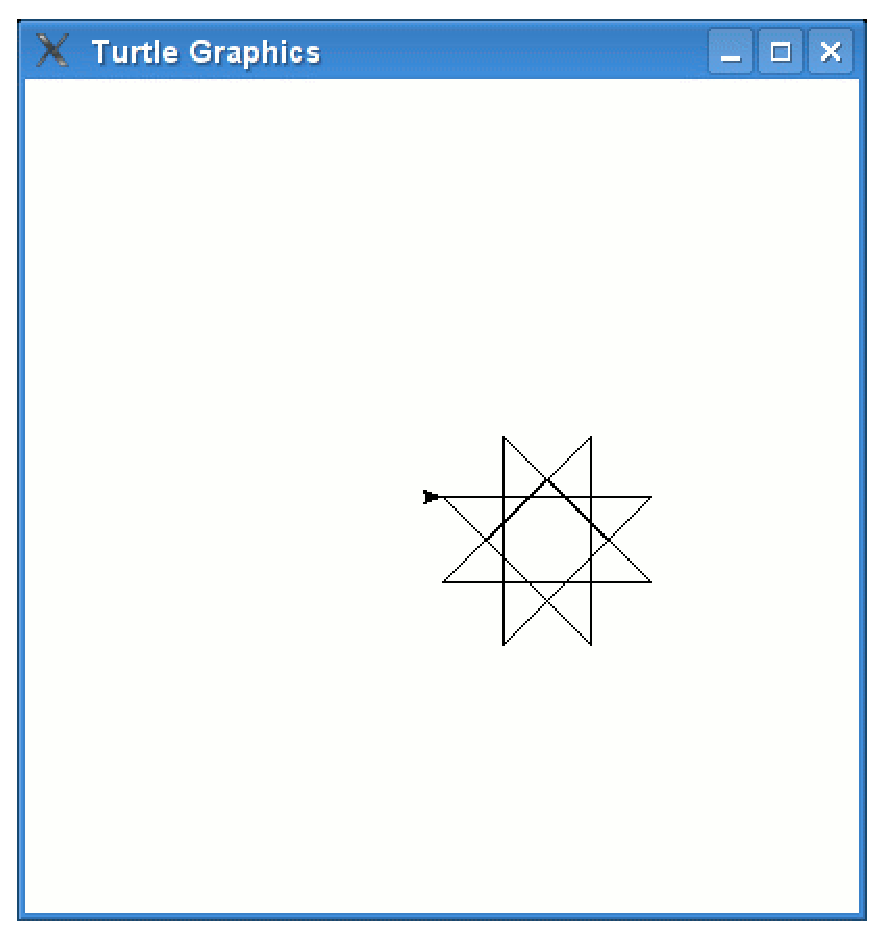
\includegraphics[width=72mm]{../en/figure20.eps}
\end{center}
\caption{Восьмиконечная звезда в исполнении черепашки.}\label{fig20}
\end{figure}

Если ещё немного поменять угол (до 175 градусов) и сделать длиннее цикл (37 шагов), то можно нарисовать звезду, у которой будет ещё больше лучей (как на картинке \ref{fig21}):

\begin{listing}
\begin{verbatim}
>>> t.reset()
>>> for x in range(1,38):
...     t.forward(100)
...     t.left(175)
...
\end{verbatim}
\end{listing}

\begin{figure}
\begin{center}
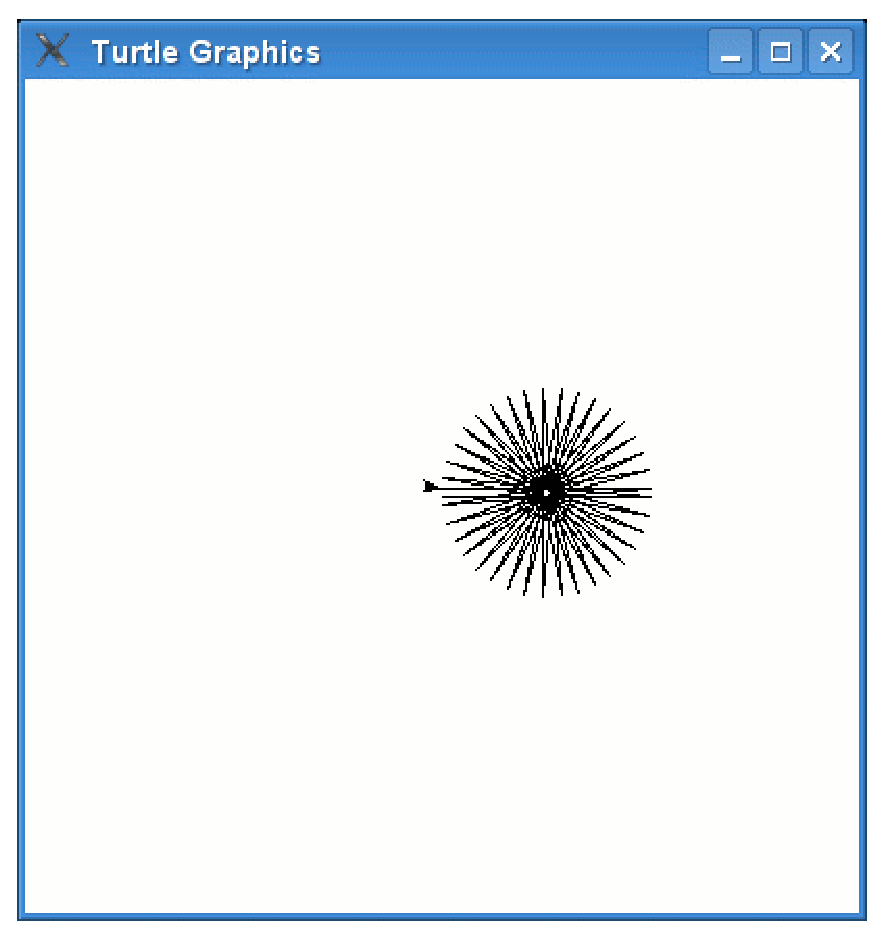
\includegraphics[width=72mm]{../en/figure21.eps}
\end{center}
\caption{Звезда, у которой много лучей.}\label{fig21}
\end{figure}

Или вот можно нарисовать что-то среднее между звездой и спиралью, как на рисунке \ref{fig22}:

\begin{listing}
\begin{verbatim}
>>> for x in range(1,20):
...     t.forward(100)
...     t.left(95)
...
\end{verbatim}
\end{listing}

\begin{figure}
\begin{center}
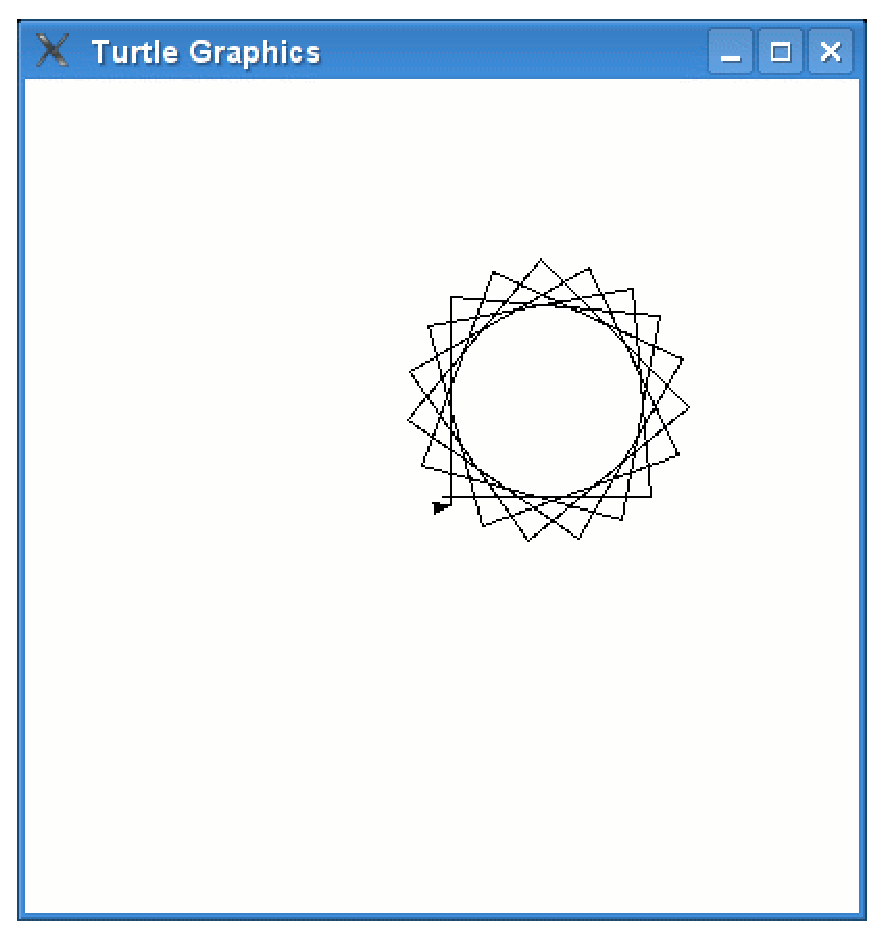
\includegraphics[width=72mm]{../en/figure22.eps}
\end{center}
\caption{Звезда с кучей лучей.}\label{fig22}
\end{figure}

Давай теперь попробуем нарисовать что-нибудь, что рисовать сложнее. Например, вот так:

\begin{listing}
\begin{verbatim}
>>> t.reset()
>>> for x in range(1,19):
...     t.forward(100)
...     if x % 2 == 0:
...         t.left(175)
...     else:
...         t.left(225)
...
\end{verbatim}
\end{listing}

В этом коде мы проверяем, содержится ли в переменной \code{x} чётное число. Для этого нам пригодится операция «\code{\%}», то есть получение остатка от деления: число ведь нечётное, если делится на два с остатком, и чётное — если без, то есть если остаток равен 0. Говоря по-питоньи, \code{if x \% 2 == 0}, то \code{x} — чётное число.

Если запустить код, который написан выше, то получится звезда с девятью лучами, как на рисунке \ref{fig23}.

\begin{figure}
\begin{center}
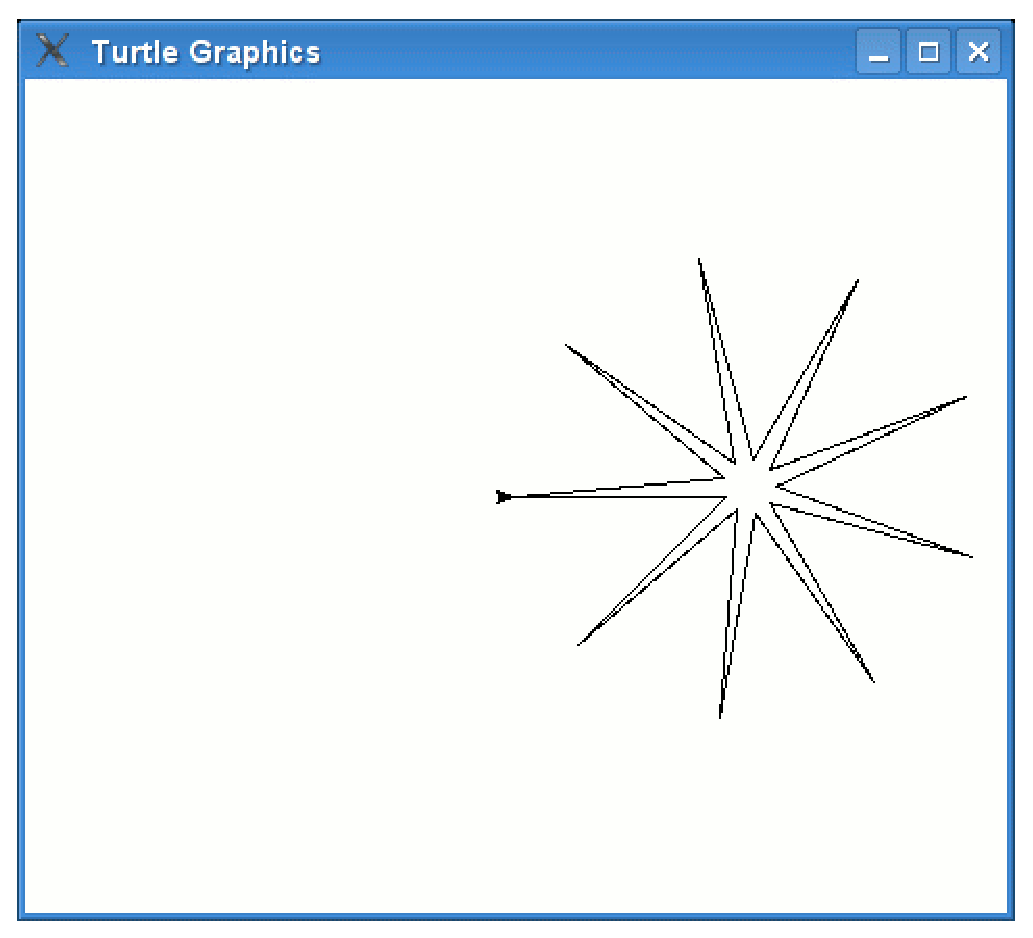
\includegraphics[width=84mm]{../en/figure23.eps}
\end{center}
\caption{Звезда с девятью лучами.}\label{fig23}
\end{figure}

Умение черепашки рисовать не ограничивается просто чёрно-белыми линиями и способностью начинать и заканчивать рисовать. Можно делать и цветные картинки, например такие:

\begin{listing}
\begin{verbatim}
t.color(1,0,0)
t.begin_fill()
t.forward(100)
t.left(90)
t.forward(20)
t.left(90)
t.forward(20)
t.right(90)
t.forward(20)
t.left(90)
t.forward(60)
t.left(90)
t.forward(20)
t.right(90)
t.forward(20)
t.left(90)
t.forward(20)
t.end_fill()
t.color(0,0,0)
t.up()
t.forward(10)
t.down()
t.begin_fill()
t.circle(10)
t.end_fill()
t.setheading(0)
t.up()
t.forward(90)
t.right(90)
t.forward(10)
t.setheading(0)
t.begin_fill()
t.down()
t.circle(10)
t.end_fill()
\end{verbatim}
\end{listing}

Код выше — долгий-долгий, утомительный и бессмысленный способ нарисовать что-то вроде машинки (она на картинке \ref{fig24}). Этот код ценен не машинкой. Он показывает, какие ещё функции есть у черепашки: \code{color} — меняет цвет фломастера, которым черепашка рисует; \code{fill} — закрашивает область на холсте всю одним цветом; \code{circle} — рисует кружочек заданного размера (диаметра).

\begin{figure}
\begin{center}
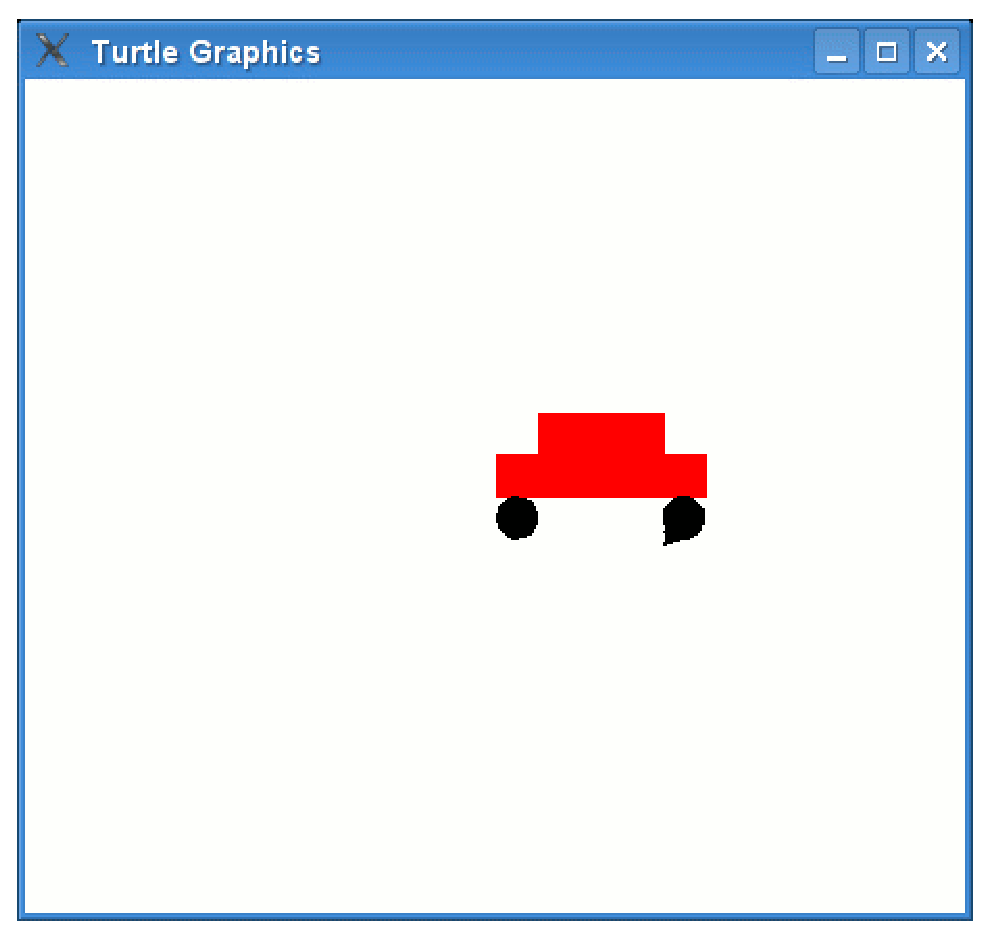
\includegraphics[width=80mm]{../en/figure24.eps}
\end{center}
\caption{Не стоит пытаться рисовать машину черепахой!}\label{fig24}
\end{figure}

\section{Добавим цвета}

Функция \code{color}\index{черепашка!color} принимает 3 параметра. Первый — интенсивность красного цвета, второй — зелёного, третий — синего.

\emph{Почему красный зелёный и синий? И что это за интенсивность такая?}

Если тебе доводилось смешивать краски, то ты можешь уже догадываться, как черепашка (и вообще, любая программа, рисующая на экране компьютера) получает цвета. Если ты смешаешь краски двух цветов, то получишь третий цвет, которым можно что-нибудь нарисовать\footnote{Когда рисуешь красками, то нужно чтобы были красный, жёлтый и синий цвета, из них можно получить любой другой. Компьютеру нужны красный, зелёный и синий, потому что на экране он рисует не красками, а наоборот, светом.}. Так, если смешать синюю и красную краски, то получится сиреневая, а если намешать слишком много красок, то может получиться серо-буро-малиновый цвет или просто какая-то коричневая грязька. В компьютере можно так же смешивать цвета: если взять одинаковое количество красного и зелёного, например, то получится жёлтый. Но в компьютере мы смешиваем цвета, которыми светит сам экран, а не цвета краски, которой мы рисуем по бумаге.

Давай на секундочку вернёмся к смешиванию краски. Представь, что у нас есть три чашки с краской. Одна чашка с красной, другая — с зелёной и третья — с синей. Каждая чашка полна краски до краёв. Так вот, если мы хотим взять целую чашку краски для получения цвета, мы должны для этого цвета передать черепашке значение 1 (то есть 100\%). Если краску из этой чашки мы брать не хотим — то значение 0. Если хотим взять полчашки, например, — то 0.5 (то есть ½). Если взять целую чашку красной и зелёной краски, то в результате получится жёлтая. Давай нарисуем жёлтый круг:

\begin{listing}
\begin{verbatim}
>>> t.color(1,1,0)
>>> t.begin_fill()
>>> t.circle(50)
>>> t.end_fill()
\end{verbatim}
\end{listing}

Тут мы вызываем функцию \code{color}, передавая ей значение 1 (100\%) для красного и зелёного цвета и 0 — для синего. Давай для дальнейших экспериментов с цветом заведём функцию, которая будет нам рисовать тем цветом, которым мы попросим:

\begin{listing}
\begin{verbatim}
>>> def draw_circle(red, green, blue):
...     t.color(red, green, blue)
...     t.begin_fill()
...     t.circle(50)
...     t.end_fill()
...
\end{verbatim}
\end{listing}

Можем нарисовать ярко-зелёный круг, взяв целую чашку зелёной краски.

\begin{listing}
\begin{verbatim}
>>> draw_circle(0, 1, 0)
\end{verbatim}
\end{listing}

А можем взять только полчашки зелёной краски…

\begin{listing}
\begin{verbatim}
>>> draw_circle(0, 0.5, 0)
\end{verbatim}
\end{listing}

…и круг получится тёмно-зелёным. Это может показаться странным: сколько краски ни возьми в реальном мире, круг всё равно будет одинаково зелёным. Но хитрость в том, что на самом деле нет. Если нарисовать тот же круг на белой бумаге, взяв мало краски, то сквозь круг будет просвечивать белая бумага, и круг будет белее, чем цвет самой краски. А компьютер, наоборот, рисует светом на чёрном экране. Мы сказали ему взять 0.5 чашки краски, то есть «половинное количество краски», и круг стал темнее, как будто сквозь него просвечивает чёрный экран.

Можешь понаблюдать за таким же эффектом, если рисовать синим и красным цветом: круг будет ярче и светлее, если «брать целую чашку краски», то есть передавать 1 в качестве значения интенсивности цвета:

\begin{listing}
\begin{verbatim}
>>> draw_circle(1, 0, 0)
>>> draw_circle(0.5, 0, 0)

>>> draw_circle(0, 0, 1)
>>> draw_circle(0, 0, 0.5)
\end{verbatim}
\end{listing}

Используя разные сочетания красного, зелёного и синего цветов, можно получить очень много цветов, почти все, которые человек может различить. Например, если смешать 100\% красного света, 85\% зелёного, и не брать синего, то получится золотистый свет:
\begin{listing}
\begin{verbatim}
>>> draw_circle(1, 0.85, 0)
\end{verbatim}
\end{listing}

А малиновый можно получить, взяв 100\% красного, 70\% зелёного и 75\% синего:

\begin{listing}
\begin{verbatim}
>>> draw_circle(1, 0.70, 0.75)
\end{verbatim}
\end{listing}

Оранжевый — взяв 100\% красного и 65\% зелёного; коричневый — 60\% красного, 30\% зелёного и 15\% синего:

\begin{listing}
\begin{verbatim}
>>> draw_circle(1, 0.65, 0)
>>> draw_circle(0.6, 0.3, 0.15)
\end{verbatim}
\end{listing}

Для того, чтобы узнать, сколько красного, синего и зелёного в нужном цвете, есть специальные программы-палитры. %
\begin{LINUX}
Например, kcolorchooser.
\end{LINUX}

И я просто напомню, что всегда можно очистить холст, написав \code{t.clear()}.

\section{Темнота}\index{turtle!color!чёрный}

Ты же знаешь, что произойдёт если ночью выключить весь свет? Всё станет чёрным.

Так и в компьютере происходит. Если не брать никакого света для рисования, то рисунок будет чёрным (цвета выключенного монитора):

\begin{listing}
\begin{verbatim}
>>> draw_circle(0, 0, 0)
\end{verbatim}
\end{listing}

Этот код рисует чёрный круг, как на картинке \ref{fig25}.

\begin{figure}
\begin{center}
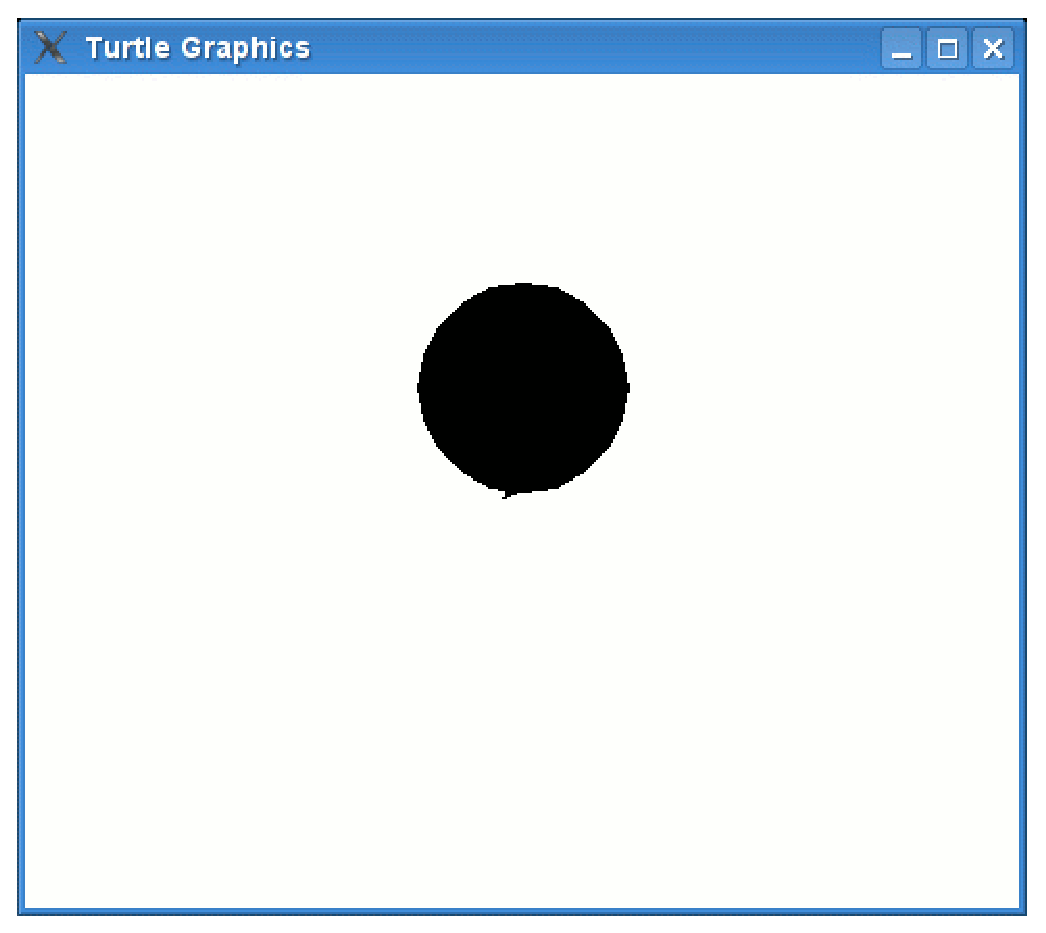
\includegraphics[width=85mm]{../en/figure25.eps}
\end{center}
\caption{Чёрная дыра!}\label{fig25}
\end{figure}

А если взять для рисования весь свет, то есть 100\% красного, 100\% зелёного и 100\% синего, то получится белый. Вот этот код уберёт обратно в небытие чёрный кружок (закрасит его белым):

\begin{listing}
\begin{verbatim}
>>> draw_circle(1,1,1)
\end{verbatim}
\end{listing}

\section{Закрашиваем рисунки}\index{черепашка!fill}

Возможно, ты уже догадался, что функция \code {begin\_fill} включает заливку цветом, а \code{end\_fill} — выключает. На самом деле, именно в момент выключения Питон и заливает нужную часть рисунка, а до тех пор только запоминает, куда потом лить краску. Зная это, мы можем нарисовать закрашенный квадрат. Вот код, который рисует просто квадрат:

\begin{listing}
\begin{verbatim}
>>> t.forward(50)
>>> t.left(90)
>>> t.forward(50)
>>> t.left(90)
>>> t.forward(50)
>>> t.left(90)
>>> t.forward(50)
>>> t.left(90)
\end{verbatim}
\end{listing}

Чтобы было проще рисовать много квадратов, да ещё и разного размера, завернём этот код в функцию:

\begin{listing}
\begin{verbatim}
>>> def mysquare(size):
...     t.forward(size)
...     t.left(90)
...     t.forward(size)
...     t.left(90)
...     t.forward(size)
...     t.left(90)
...     t.forward(size)
...     t.left(90)
\end{verbatim}
\end{listing}

Всё ли вышло успешно? Давай проверим.

\begin{listing}
\begin{verbatim}
>>> mysquare(50)
\end{verbatim}
\end{listing}

У меня квадрат нарисовался.

\emph {…в воображении. В книге нет консоли питона, но даже у книги есть воображение.}

Если присмотреться к этому коду, можно заметить, что в нём кучу раз повторяются одни и те же две строки. А если ещё пристальнее присмотреться, то даже удастся сосчитать, сколько раз они повторяются: четыре. Так что тут хорошо бы смотрелся цикл — вот такой:

\begin{listing}
\begin{verbatim}
>>> def mysquare(size):
...     for x in range(0,4):
...         t.forward(size)
...         t.left(90)
\end{verbatim}
\end{listing}

Можешь попробовать нарисовать квадратов всякого разного размера:

\begin{listing}
\begin{verbatim}
>>> t.reset()
>>> mysquare(25)
>>> mysquare(50)
>>> mysquare(75)
>>> mysquare(100)
>>> mysquare(125)
\end{verbatim}
\end{listing}

Должно получиться что-то вроде рисунка \ref{fig26}.

\begin{figure}
\begin{center}
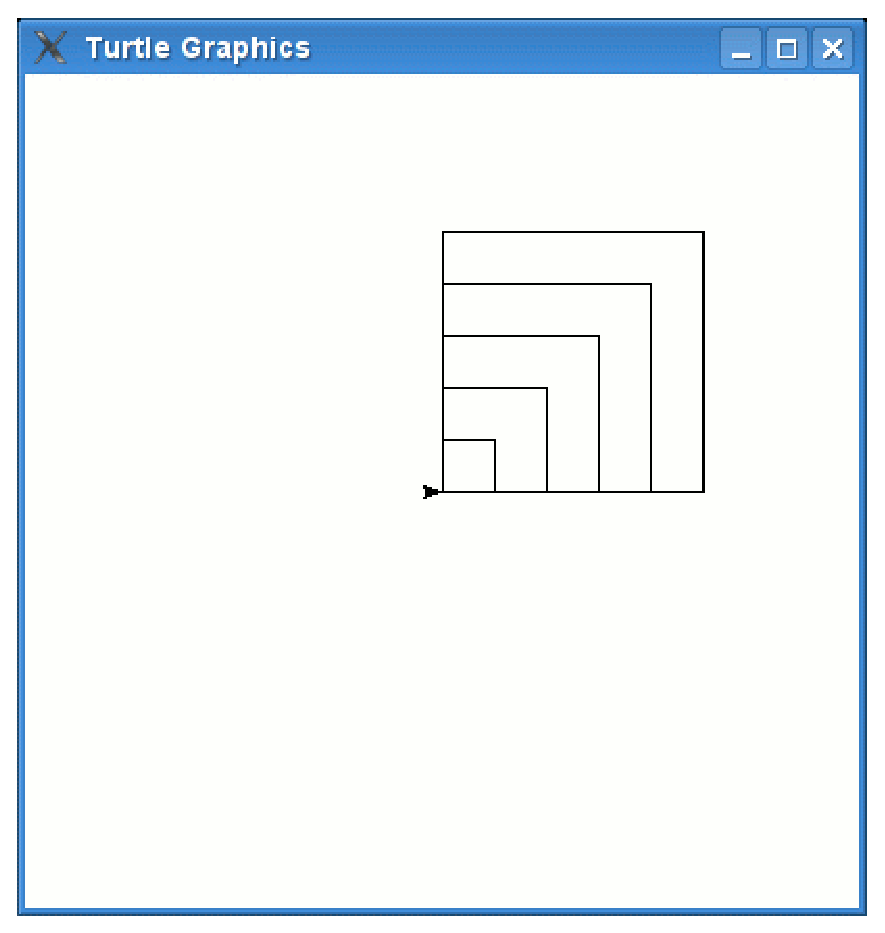
\includegraphics[width=72mm]{../en/figure26.eps}
\end{center}
\caption{Квадратики. Много.}\label{fig26}
\end{figure}

Ну а теперь можно приступить к рисованию закрашенных квадратов. Прежде всего, надо очистить холст от тех шедевров, что на нём уже есть:

\begin{listing}
\begin{verbatim}
>>> t.reset()
\end{verbatim}
\end{listing}

Потом включить заливку и нарисовать квадрат:

\begin{listing}
\begin{verbatim}
>>> t.begin_fill()
>>> mysquare(50)
\end{verbatim}
\end{listing}

…и потом наконец закрасить нарисованное:

\begin{listing}
\begin{verbatim}
>>> t.end_fill()
\end{verbatim}
\end{listing}

В результате получается картинка \ref{fig27}.

\begin{figure}
\begin{center}
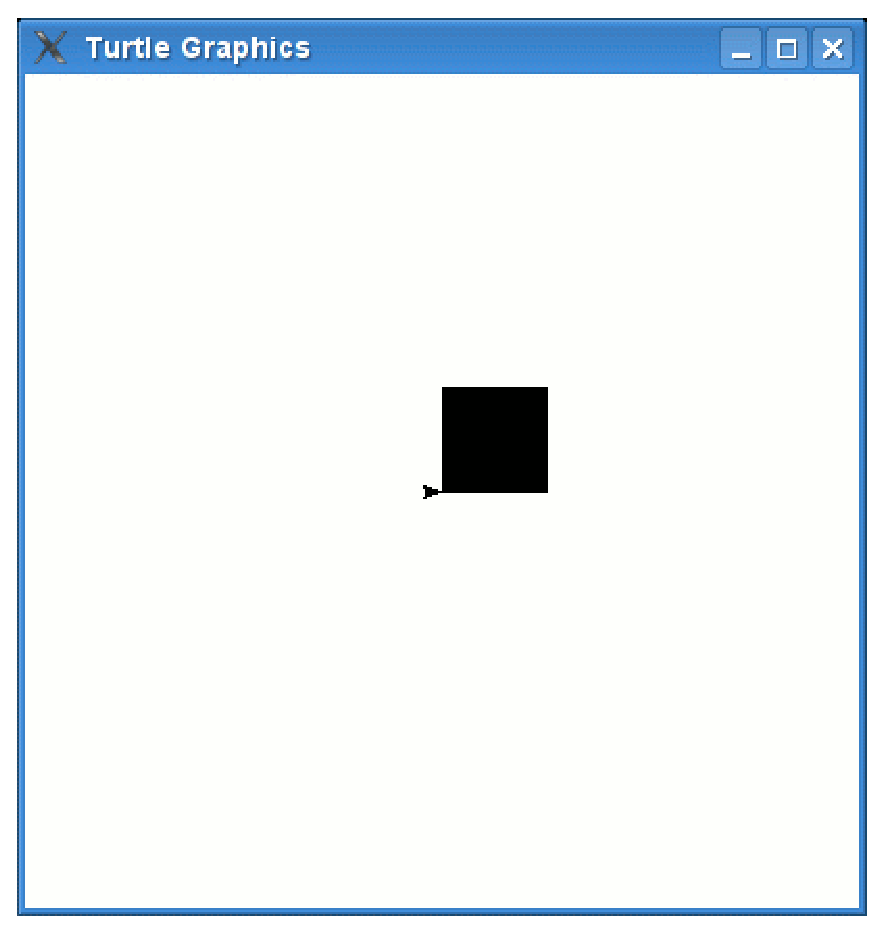
\includegraphics[width=72mm]{../en/figure27.eps}
\end{center}
\caption{Чёрный квадрат.}\label{fig27}
\end{figure}

Можно сделать рисование закрашенных квадратов чуточку удобнее: добавить в функцию рисования квадрата параметр, в зависимости от которого квадрат будет получаться или закрашенным, или нет:

\begin{listing}
\begin{verbatim}
>>> def mysquare(size, filled):
...    if filled == True:
...        t.begin_fill()
...    for x in range(0,4):
...        t.forward(size)
...        t.left(90)
...    if filled == True:
...        t.end_fill()
...
\end{verbatim}
\end{listing}

Первые две строки проверяют, равна ли переменная \code{filled} «истине» (\code{True} по-английски), то есть просили ли нас закрашивать. Если да, то включается заливка цветом. Потом рисуется квадрат, потом заливка завершается, если нас вообще просили закрашивать. Теперь закрашенный квадрат можно нарисовать так:
\begin{listing}
\begin{verbatim}
>>> mysquare(50, True)
\end{verbatim}
\end{listing}

…а не закрашенный — вот так:

\begin{listing}
\begin{verbatim}
>>> mysquare(150, False)
\end{verbatim}
\end{listing}

И результат получается, как на рисунке \ref{fig28}… мне он напоминает безумный квадратный глаз.

\begin{figure}
\begin{center}
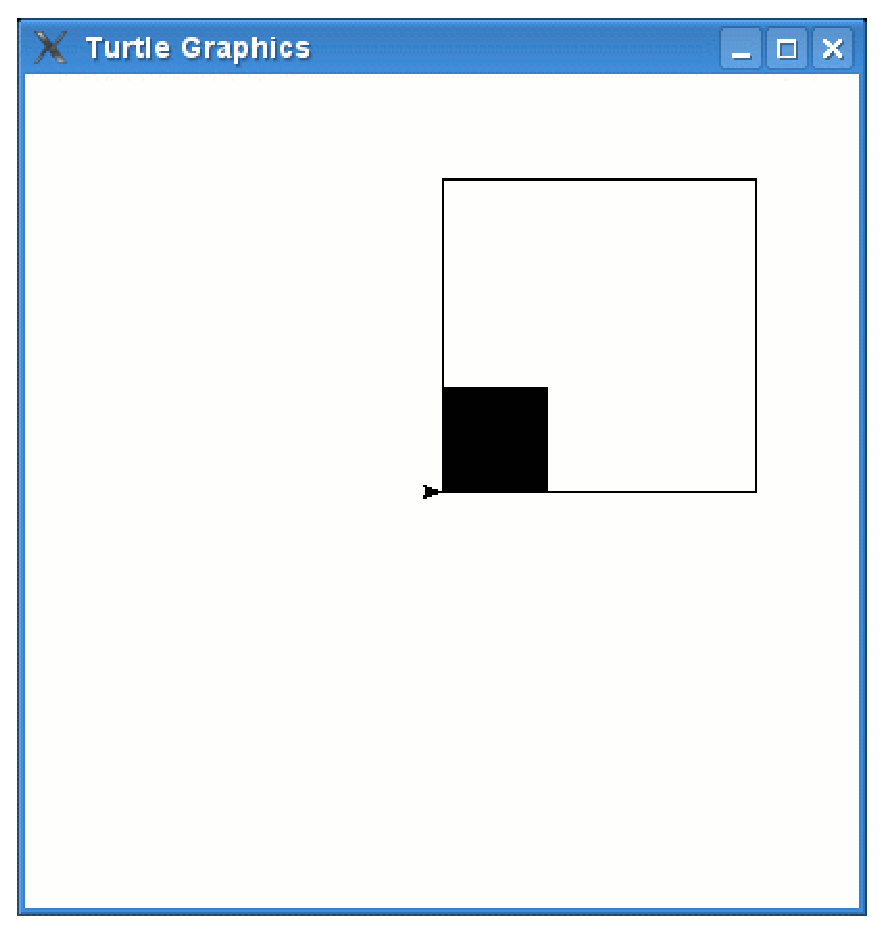
\includegraphics[width=72mm]{../en/figure28.eps}
\end{center}
\caption{Квадратный глаз}\label{fig28}
\end{figure}

Примерно так можно рисовать и всё остальное, что в голову взбредёт, и закрашивать цветом. Например, можем сделать функцию рисования звезды, которую мы в начале главы рисовали:

\begin{listing}
\begin{verbatim}
>>> for x in range(1,19):
...     t.forward(100)
...     if x % 2 == 0:
...         t.left(175)
...     else:
...         t.left(225)
...
\end{verbatim}
\end{listing}

Заворачиваем это в функцию, добавляем параметр, указывающий, надо ли закрашивать звезду (и ещё размер добавим, как для квадрата тоже), и получаем такой код:

\begin{listing}
\begin{verbatim}
1.  >>> def mystar(size, filled):
2.  ...     if filled:
3.  ...         t.begin_fill()
4.  ...     for x in range(1,19):
5.  ...         t.forward(size)
6.  ...         if x % 2 == 0:
7.  ...             t.left(175)
8.  ...         else:
9.  ...             t.left(225)
10. ...     if filled:
11. ...         t.end_fill()
\end{verbatim}
\end{listing}

Давай теперь проверим, что эта функция на самом деле делает: попробуем нарисовать золотистую звезду:

\begin{listing}
\begin{verbatim}
>>> t.color(1, 0.85, 0)
>>> mystar(120, True)
\end{verbatim}
\end{listing}

Черепашка должна изобразить рисунок \ref{fig29}. Теперь давай добавим к этой звезде чёрный контур: поменяем цвет, выключим заливку и нарисуем звезду того же размера ещё раз:

\begin{figure}
\begin{center}
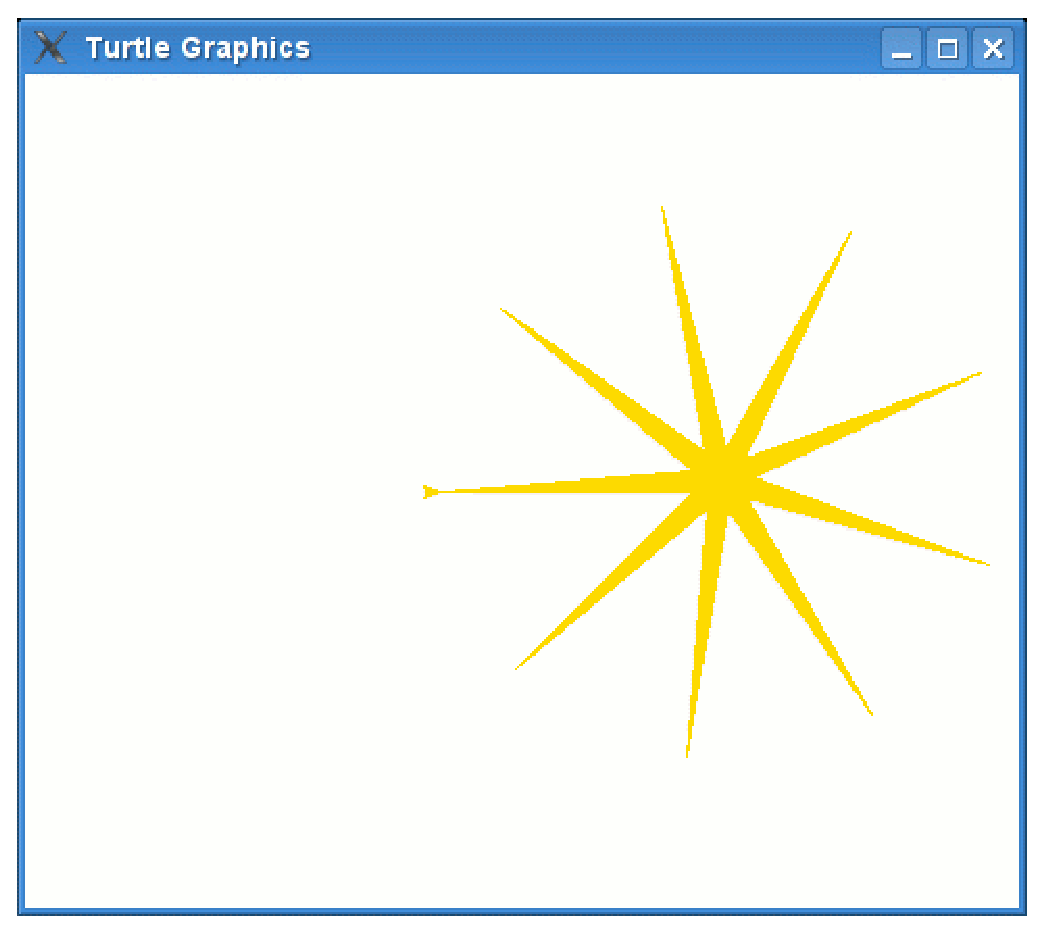
\includegraphics[width=85mm]{../en/figure29.eps}
\end{center}
\caption{Золотая звезда.}\label{fig29}
\end{figure}

\begin{listing}
\begin{verbatim}
>>> t.color(0,0,0)
>>> mystar(120, False)
\end{verbatim}
\end{listing}

Теперь звезда должна выглядеть так: \ref{fig30}.

\begin{figure}
\begin{center}
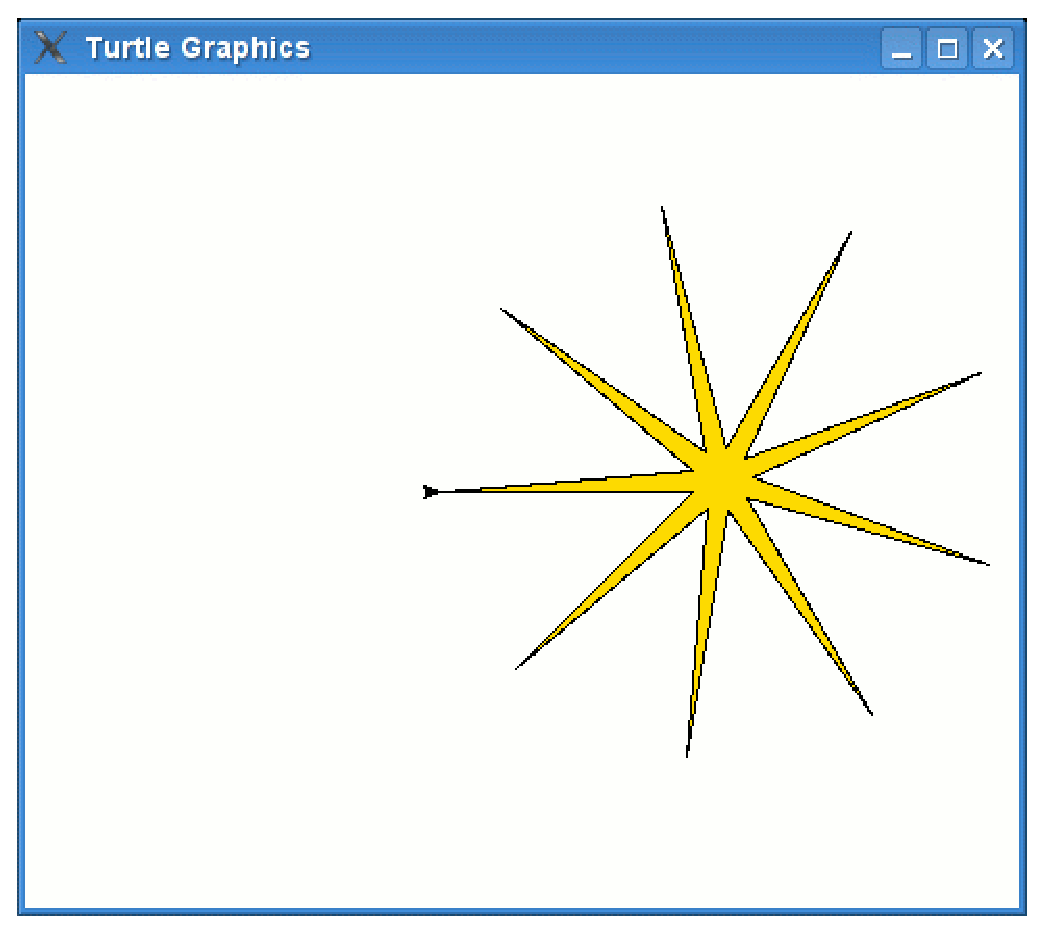
\includegraphics[width=85mm]{../en/figure30.eps}
\end{center}
\caption{Звёздочка с контуром.}\label{fig30}
\end{figure}

\section{Как ещё развлечься}

\emph{В этой главе мы посмотрели на разные функции черепашки — модуля turtle Питона — и с её помощью нарисовали некоторые геометрические фигуры. Мы создали функции для рисования фигур, а также для закраски их цветом.}

\subsection*{Упражнение 1}
Ну хорошо, вот мы нарисовали звёздочки, квадратики, прямоугольники. А как насчёт восьмиугольника? Попробуй нарисовать его. (Поворачивай на 45 градусов, это ключ к успеху).

\subsection*{Упражнение 2}
Создай функцию для рисования закрашенных и не закрашенных восьмиугольников разного размера.

\newpage
